This layer processes the data scanned from the presentation layer and stores the data in local variables, i.e. name 
of the beverage and expiry date. This data is added to the current user's beverage database and send the updated data
back to the presentation layer for further input.

\begin{figure}[h!]
	\centering
 	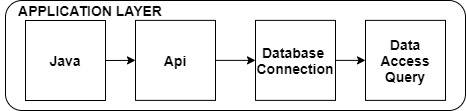
\includegraphics[width=0.60\textwidth]{images/App.jpg}
 \caption{Example subsystem description diagram}
\end{figure}

\subsection{Java Subsystem}
The Java Subsystem is responsible for taking the XML data provided from the Presentation layer and and send it to the API 
subsystem to connect to the dataset and accurately get the required information. After the data is retrieved from the dataset,
this subsystem passes the result to the Response subsystem in the Presentation layer.

\subsubsection{Assumptions}
\begin{itemize}
    \item The xml input is in the proper format.
\end{itemize}

\subsubsection{Responsibilities}
The application must successfully connect to the database.

\subsubsection{Subsystem Interfaces}

\begin {table}[H]
\caption {Subsystem interfaces} 
\begin{center}
    \begin{tabular}{ | p{1cm} | p{6cm} | p{3cm} | p{3cm} |}
    \hline
    ID & Description & Inputs & Outputs \\ \hline
    \#1 & XML to Java & \pbox{XML file} & \pbox{API}  \\ \hline
    \#2 & SQLite3 to Java & \pbox{Beverage Data} & \pbox{Formatted Data}  \\ \hline
    \#3 & Java to Response & \pbox{Formatted Data} & \pbox{}  \\ \hline
    \end{tabular}
\end{center}
\end{table}


\subsection{API Subsystem}
The API subsystem passes the barcode to the Data Access Layer and retrieves the information of the beverage being 
scanned. The data retrieved is added to the current dataset of beverages which the user owns. 

\subsubsection{Assumptions}
\begin{itemize}
    \item The API exists in the dataset.
\end{itemize}

\subsubsection{Responsibilities}
The API must be able to establish fetch data on the database.

\subsubsection{Subsystem Interfaces}

\begin {table}[H]
\caption {Subsystem interfaces} 
\begin{center}
    \begin{tabular}{ | p{1cm} | p{6cm} | p{3cm} | p{3cm} |}
    \hline
    ID & Description & Inputs & Outputs \\ \hline
    \#1 & Java to API & \pbox{Product ID} & \pbox{API fetche call}  \\ \hline
    \end{tabular}
\end{center}
\end{table}



\subsection{Database Connection Subsystem}
This subsystem establishes the connection between the database (Firebase) and the application. 

\subsubsection{Assumptions}
\begin{itemize}
    \item A database is present and operational.
\end{itemize}

\subsubsection{Responsibilities}
The connection must be present at all times to allow for the various features to be implemented properly. 

\subsubsection{Subsystem Interfaces}

\begin {table}[H]
\caption {Subsystem interfaces} 
\begin{center}
    \begin{tabular}{ | p{1cm} | p{6cm} | p{3cm} | p{3cm} |}
    \hline
    ID & Description & Inputs & Outputs \\ \hline
    \#1 & API to Database & \pbox{API call} & \pbox{Database connection}  \\ \hline
    \end{tabular}
\end{center}
\end{table}



\subsection{Data Access Query Subsystem}
This will fetch the data being query as per the API request and send the result back to the application.

\subsubsection{Assumptions}
\begin{itemize}
    \item The query is always valid.
\end{itemize}

\subsubsection{Responsibilities}
Must return the correct data as per the query.

\subsubsection{Subsystem Interfaces}

\begin {table}[H]
\caption {Subsystem interfaces} 
\begin{center}
    \begin{tabular}{ | p{1cm} | p{6cm} | p{3cm} | p{3cm} |}
    \hline
    ID & Description & Inputs & Outputs \\ \hline
    \#1 & Query to Database & \pbox{Data in the dataset} & \pbox{JSONified data}  \\ \hline
    \end{tabular}
\end{center}
\end{table}
